\section{Research Workflow}
this is a workflow section
\section{Required Installation and Configuration}
The research purposes a solution based on deep convolutional neural networks
With various experiments mentioned in further sections.  The experiments
require specific configuration for cuda libraries to run programs on available GPU(Graphical Processing Unit) for faster processing
and further, instructions to setup environment can be found at Tensorflow gpu installation guide \footnote[1]{\url{https://www.tensorflow.org/install/gpu}}.
Alternatively, the machine learning models can also run without installing cuda libraries on CPU but the processing will be slow.
In addition, the convolutional neural network was implemented using Python3 and Jupyter notebooks were used in these experiments which provides an appropriate interface to experiment and write markdowns.  
Jupyter notebooks can be installed by installing Anaconda \footnote[2]{https://www.anaconda.com/distribution/}.
Furthermore, data science and machine learning libraries are required such as Numpy, Keras, Matplotlib and OpenCV. 
Numpy library is required for performing mathematical operations on multi-dimensional NumPy arrays. The matplotlib library provides an interface to visualise the output results. 
The OpenCV library was used for image processing in the process of developing an automated system for classifying
pigmented skin lesions. Moreover, keras library was used to develop deep convolutional models. 
HAM,1000 (Human Against Machine, 1000) dataset was used to develop image classifier \citep{DVN/DBW86T_2018}.
The dataset primarily contains two folders which includes overall 10,000 dermatoscopic images of pigmented skin lesion. In addition, it also contains a csv file which includes the meta-information regarding pigmented skin lesions.
The required files can be downloaded from harvard dataverse webiste \footnote[3]{\url{https://dataverse.harvard.edu/dataset.xhtml?persistentId=doi:10.7910/DVN/DBW86T}}.

\pagebreak
\section{Data Processing and Normalisation}
\begin{figure} [!htp]
    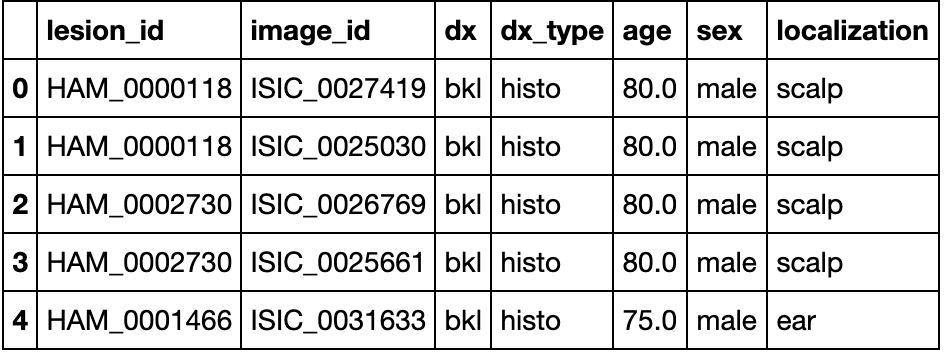
\includegraphics[width=\textwidth]{Images/datae.png}
    \caption{Pandas Dataframe containing information about pigmented skin lesions}
    \label{fig:pandasTop}
\end{figure}

The information was read using pandas into the data frame, 
which is a data structure that allows storing tabular data from CSV files as showm in 
figure \ref{fig:pandasTop}.The CSV file contained irrelevant information such as sex, age and localisation 
of patients in the data frame which was removed by dropping the non esential columns.
In addition, the dataset contains unclear and hairy images of pigmented skin lesions which were manually 
removed from the dataset to enhance the quality of available data.
Furthermore, the research only focuses on limited categories of 
pigmented skins which results in dropping data columns for the other categories 
of data. The information shown in above dataframe contains a lesionid column which coresponds
to image names which were were read into numpy array using pillow library from respective directories.
The data for convolutional neural networks needs to divided into training and testing data, the model learnings
are peformed with learning the patterns and relationships in the training datasets and evaluation of the 
model is performed on the testing data which is never feed to the intelligent model which training.
The dataset was divided into training and testing sets using \url{sklearn.model_selection.train_test_split} class in the portion of 80 per cent for 
the training dataset and 20 per cent of testing datasets. The next step towards to preparing the dataset was reading the images data into NumPy 
array for both training and testing datasets and converting the image names from pandas series to NumPy array corresponding to each image and assign class number 
based on category of pigmented skin lesion in the dataset. Furthermore, the training and testing datasets were serialised into 
dictionary in a pickle encoded file. Therefore, the encoded file sizes are compact and are portable
in comparison to storing actual image files.
\subsection{Data Normalisation}
The images with RGB(Red, Green and Blue) channels information was stored in numpy mutli-demensional array with numbers ranging from 0 to 255.
The numpy array was converted into the float32 format and each element of the array was divided by 255 to normalise the data so, that 
it only ranges between 0 and 1 in float format which will help while training the model. In addition, one hot encoding 
was performed on class labels of the pigmented lesions. The one hot encoding is a representation of categorical variable 
as binary vector and normalise the categorical labels into binary vector.
\subsection{ Image Segmentation }
\begin{center}
	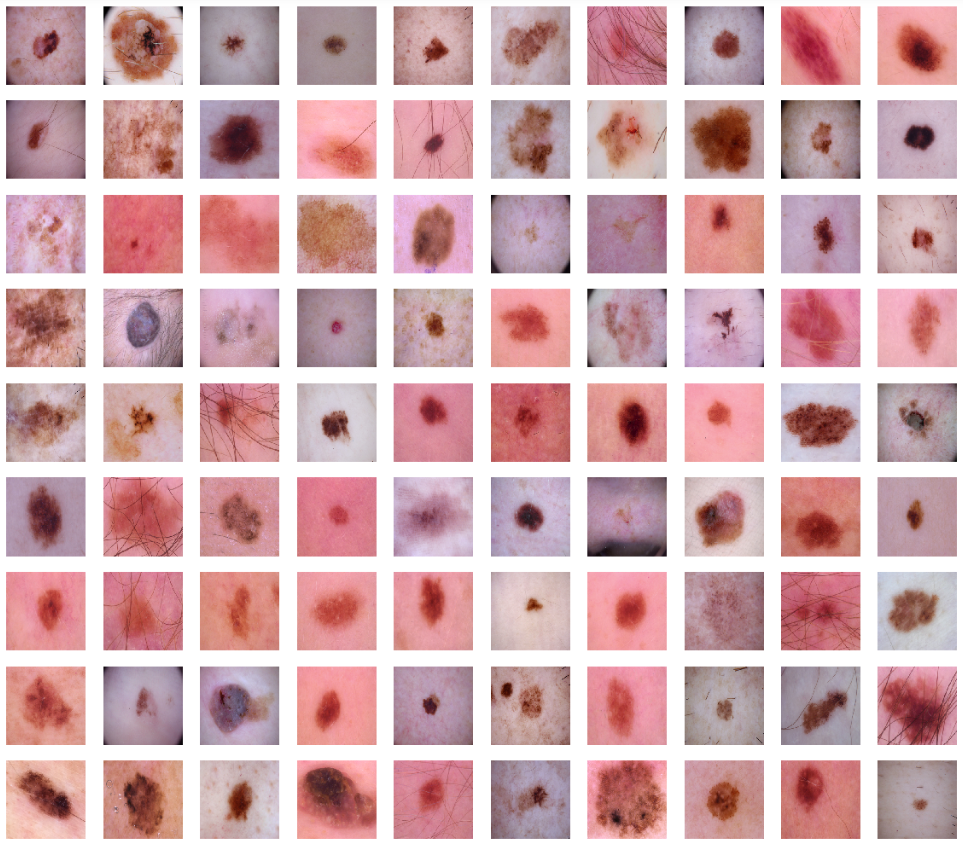
\includegraphics[width=10cm]{Images/bseg.png}
\end{center}

The figure above reflects the sample from training dataset before performing image segmentation.
The image segmentation was performed on the all the images using binary thresholding in OpenCV framework.

\section{Thresholding Segmentation Algorithm}

Thresholding is one of the commonly adopted method in image segmentation which helps in descrimination most 
significant pixels in the images \citep*{al2010image}. The thresold value is selected and the gray scale images  
are converted into the binary representation of the image and value of image which are greater than the thresold
value will be selected with keeping all the attributes of the images such as position and shape \citep*{al2010image}. 
Thus, reducing the complexity of the image data and making it easier for classification related tasks. Futhermore, the 
segmented images will be consumed in the model training. The thresholding segmentation was performed using OpenCV library using 
\url{cv.threshold(image, 0.5, 1, cv.THRESH_BINARY)} where threshold value of 0.5 and maximum value of the pixel can be 1
as it was normalised.

\begin{center}
	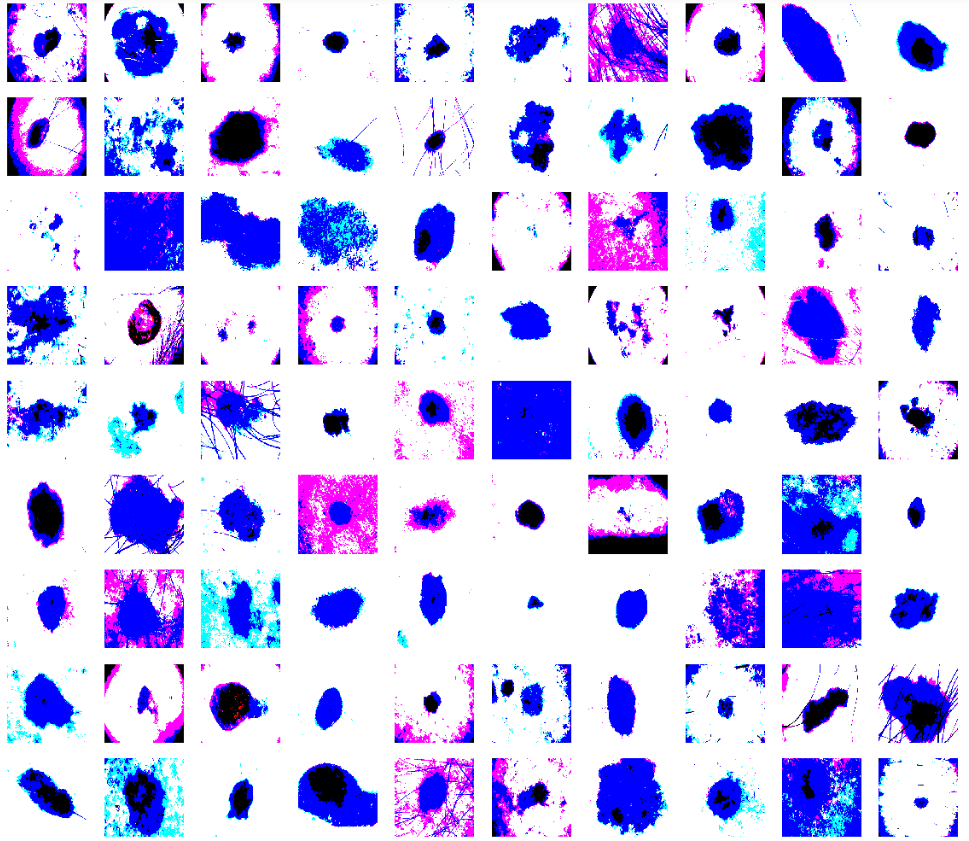
\includegraphics[width=10cm]{Images/aseg.png}
\end{center}

The figure above shows the result of applying the threshold image segmentation on pigmented skin lesions. 

\pagebreak
\section{Convolutional Model Training}
\begin{figure}[!htp]
    \centering
    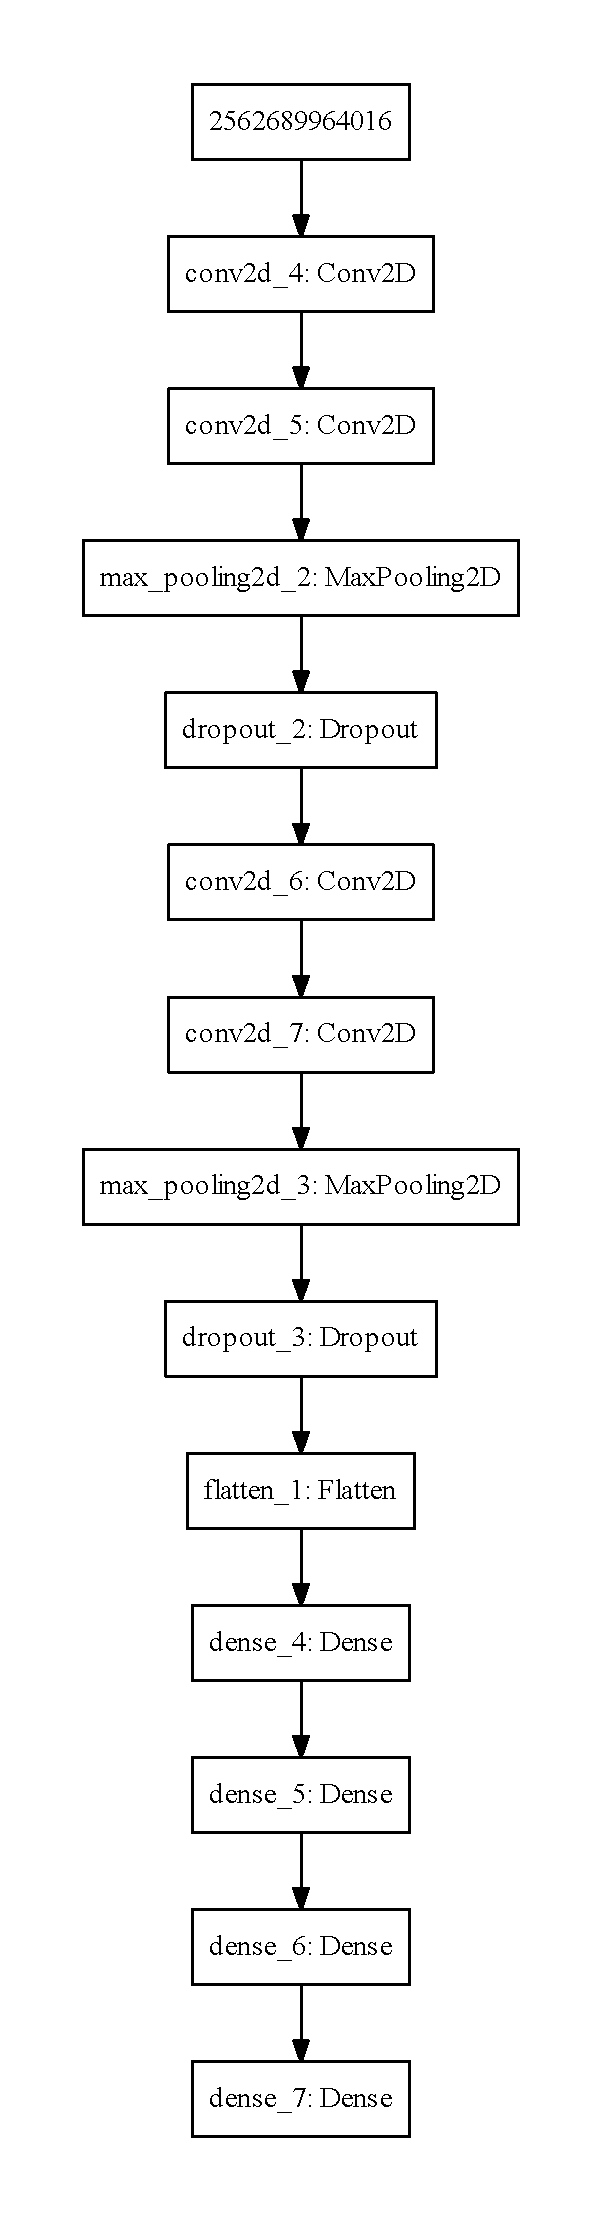
\includegraphics[height=.8\textheight]{Documents/model.pdf}
    \caption{Model Architecture 1}
    \label{fig:model1}
\end{figure}
The model architecture \ref{fig:model1} was implemented using the keras Api in which 2 dimensional 
convolutional layers were added to the sequantial network with intial dimension of image in (224, 224, 3), where width and height of input image is 224 pixels and the rgb channels depth 
are represented by 3. The initial convolutional layers contains 32 input filters with the kernel size of (3, 3) with relu 
activation function. In the network layers followed by first two convolutional layers are polling layer in the 
architecture MaxPooling was used to extract maximum of the input features after applying image filter or kernel 
to the given image of pigmented skin lesions. Furthermore, dropout of 0.4 was used in the network to generialise the 
overall performance of the network and avoid overfitting of data points. 
The next two layers in the networks are also another convolutional layers with 64 image filters and similar relu activation function. Similar fashion as aboved was 
applied to the network with MaxPooling to extract most significant pixels from feature maps followed by the dropout in the network to generialise it.
The features extracted by the convolutional layers are flattened into one dimensional array. The flattened array will be passed to the fully connected layers in the neural network
to process the information. The model contains three dense hidden layers and one output layer in the neural network.
Furthermore, the model architecture was compiled using various hyper-parameters which effects such as learning rate and 
optimiser for the convolutional model which helps in computing the gradient for the loss function to minimise the error in predecting 
category of pigmented skin lesion.

\subsection{Experiments for optimal Model optimiser}
The model architecture at initial stages was compiled using different hyper-parameters
such as optimal optimiser for the neural network and learning rate. These 
hyper-parameters can have impact in finding gradient descent of loss function. Keras libraries 
provides various optimisers such as Adam, SGD and RMSProp Optimiser which 
aims towards reducing the cost function. The model architecture mentioned above was trained for 30 epochs or iteration to 
investigate the optimal optimiser for classification of pigmented skin lesions. The model was trained under learning 
constant rate of 0.001 and loss function of categorical crossentropy because the model has to evaluate the mutiple data classes 
for pigmented skin lesions.

\pagebreak

\begin{figure}[!htp]
    \centering
    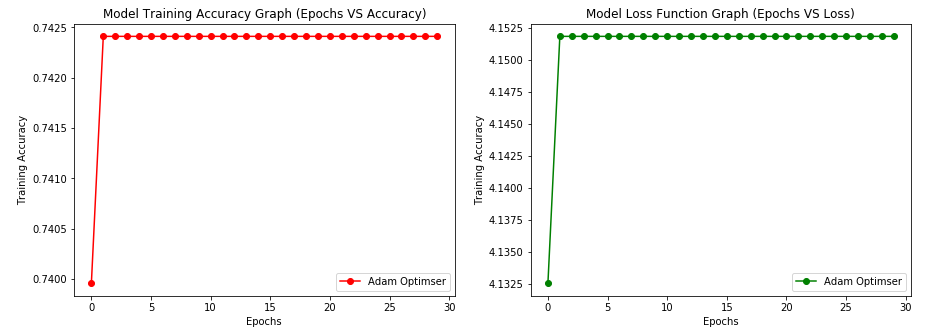
\includegraphics[width=15cm]{Images/Adam Optimiser.png}
    \caption{Model Results obtained with Adam Optimiser}
    \label{fig:adam}
\end{figure}

\paragraph{Adam Optimiser}
The figure \ref{fig:adam} refects the results obtained from training the model using adam optimiser. The figure \ref{fig:adam} shows that model loss function 
is not decreasing and after few epochs there was no improvment in model accuracy which means that adam optimiser is sutaible 
optimiser for model architecture \ref{fig:model1} presented above.

\begin{figure}[!htp]
    \centering
    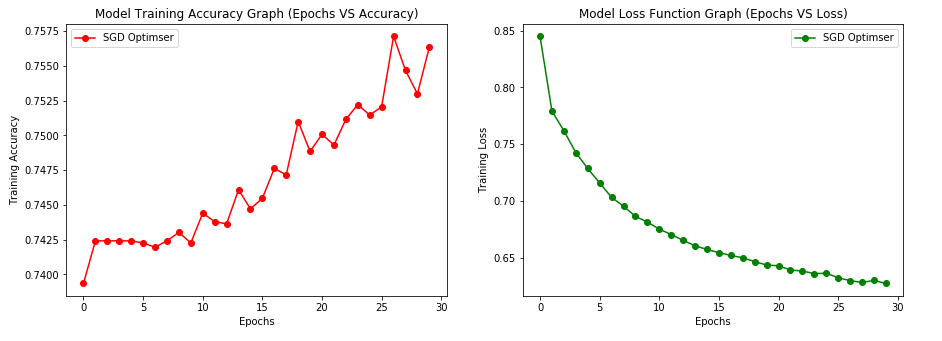
\includegraphics[width=15cm]{Images/SGD.png}
    \caption{Model Results obtained with SGD Optimiser}
    \label{fig:sgd}
\end{figure}

\paragraph{SGD Optimiser}
The figure \ref{fig:sgd} refects the results obtained from training the model using sgd optimiser. The model shows improvment in model 
performance. The training accuracy of model increased over epochs and loss function was decreasing as anticipated as shown in the figure 
\ref{fig:sgd} above.


\begin{figure}[!htp]
    \centering
    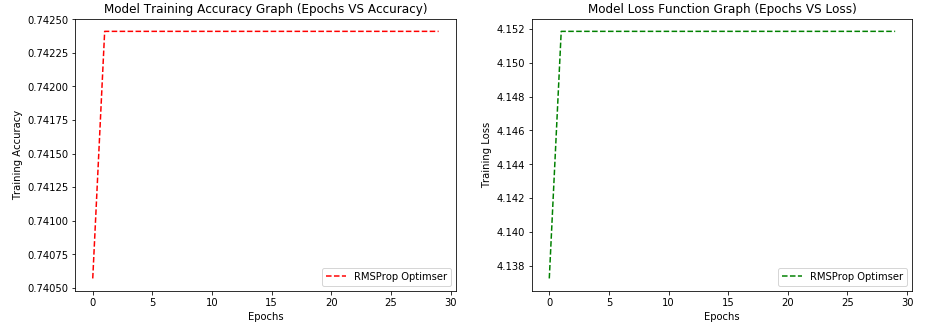
\includegraphics[width=15cm]{Images/rmsprop.png}
    \caption{Model Results obtained with RMSProp Optimiser}
    \label{fig:rms}
\end{figure}

\paragraph{RMSProp Optimiser}
The figure \ref{fig:rms} refects the results obtained from training the model using 'RMSProp' optimiser. The model performance was similar to 
the adam optimiser.Therefore, the SGD optimiser was optimial optimiser for classificaiton model under the constant hyper parameters mentioned above.
the further, experiments performed on convolutional neural network are trained on SGD optimiser.

\section{Model Experiments with Learning Rates}

\begin{figure}[!htp]
    \centering
    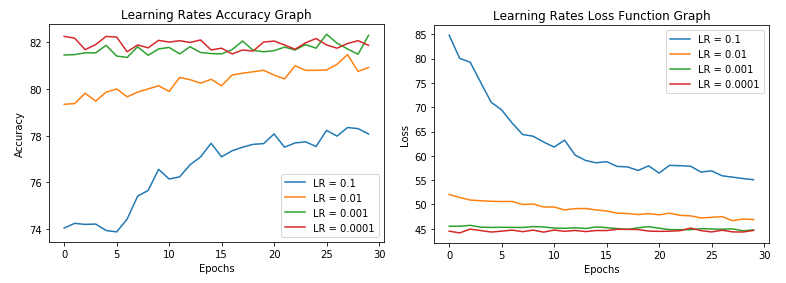
\includegraphics[width=15cm]{Images/lr.png}
    \caption{Model Results obtained with different learning rates}
    \label{fig:lrates}
\end{figure}




\pagebreak
\section{Experiments with Hyperparameters}
The experiments were performed on the convolutional model to understand the effects of the hyper-parameters 
such as learning rate of the network, the number of epochs for which the model for trained and increasing the hidden  
and convolutional layers. The adjustments to the hyperparameters which were made on the model had an impact on the accuracy of the overall classification of the pigmented skin lesions.
\subsection{Learning Rate Experiment}
\begin{figure}[!htp]
    \centering
    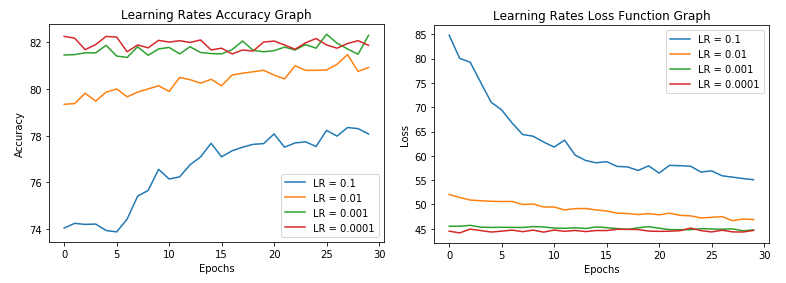
\includegraphics[width=15cm]{Images/lr.png}
    \caption{Variable Learning Rates}
    \label{fig:lrates}
\end{figure}

The figure \ref{fig:lrates} above shows that the model was trained for different learning rates as shown
in the legend of the figure \ref{fig:lrates} for thirty epochs or iterations. The outcome of the above test 
was that the model model accuracy of the model were increasing with decrease in the learning rates. Thus, it 
can be concluded that the model accuracy was  inversely proportional to the learning rate. The figure \ref{fig:lrates} also shows the 
decline in the loss function where learning rate was found directly proportional to loss function of the 
convolutional model. Therefore, the most optimal learning rate to train the convolutional network 
neural network was 0.0001. However, the model with the lower the learning rate consumes more time in the 
process of training. Further model training experiments are peformed on 
learning rate of 0.001 to achieve the accuracy and realtive speed to train the model.



\subsection{Epochs Experiment}
\begin{figure}[!htp]
    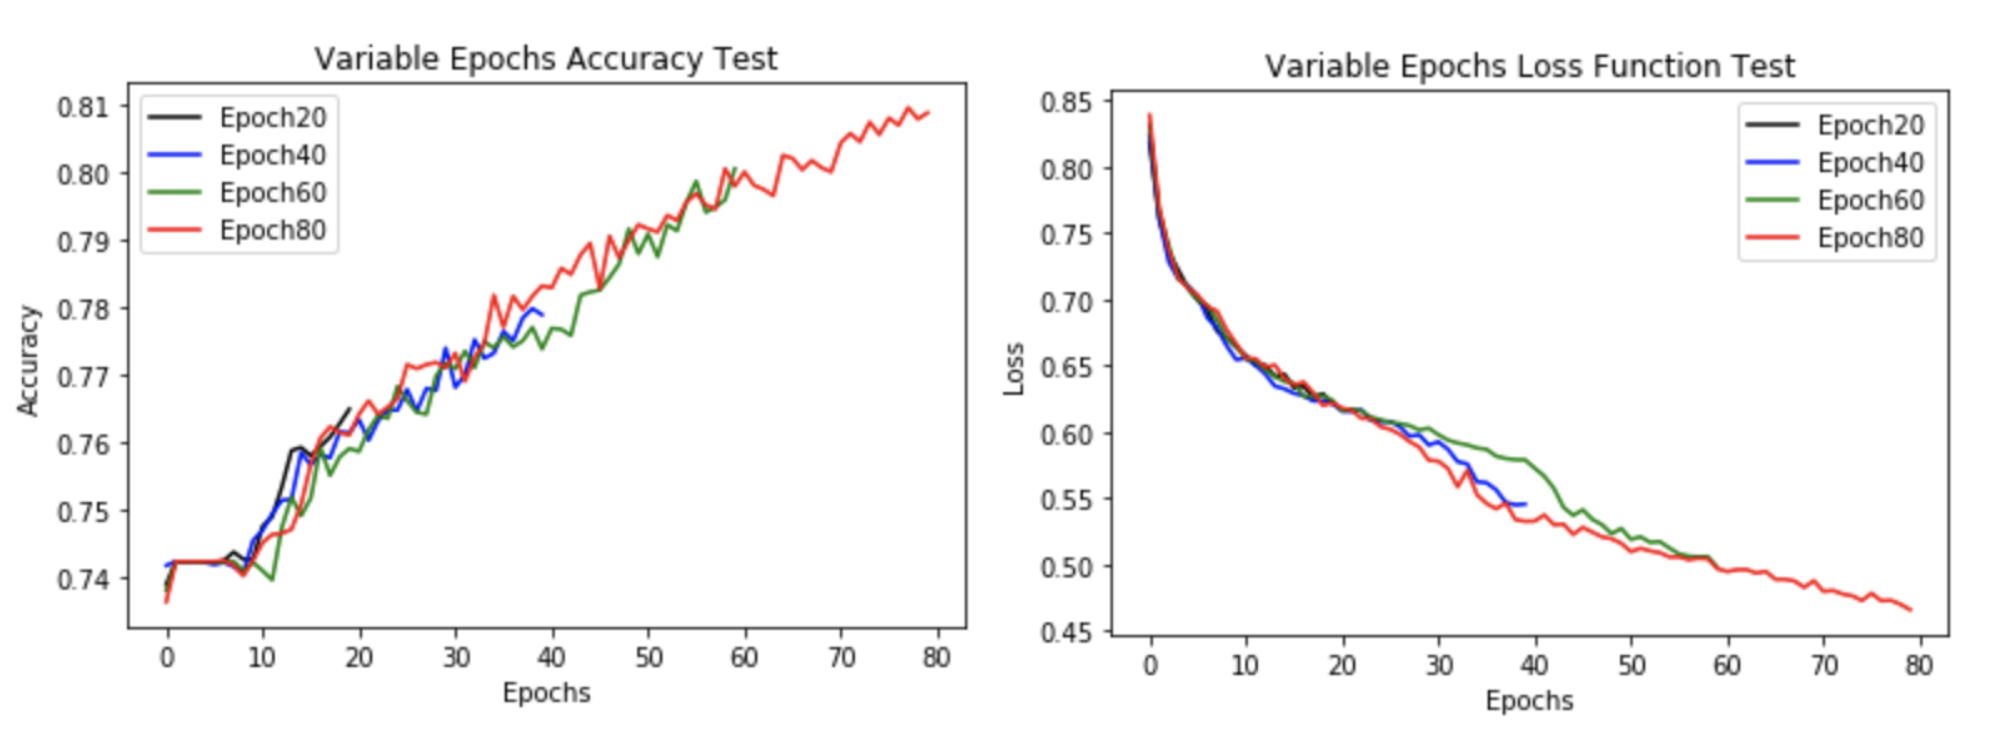
\includegraphics[width=\textwidth]{Images/epochs.png}
    \caption{Results obtained different epochs}
    \label{fig:epochsTest}
\end{figure}

The figure \ref{fig:epochsTest} shows the accuracy of model with same architecture for 
different number of epochs. The model accuracy is directly proptional the number of epochs as 
training the nural networks is optimisation problem and objective is to find minimum of the cost 
function. The model accuracy on training data improves over each epoch as the model finds 
local minimum of cost function at each epoch and improve the predection in the next iteration.
However, when the model reaches the gloabal minimum of the objective function there will 
be improvments in model accuracy. The figure \ref{fig:epochsTest} shows the model trained 
with the most number of epochs which is eighty in these experiments has least value of 
cost function and maximum training accuracy.

\begin{center}
    \begin{tabular} { | c | c | c | c |}
        \hline
        Learning Rate & Test Accuracy & Epochs  & Optimiser\\ 
        \hline
        0.01 & 73.61\% & 20 & SGD \\ 
        \hline 
        0.01 & 76.97\% & 40 & SGD  \\
        \hline 
        0.01 & 79.46\% & 60 & SGD \\
        \hline
        0.01 & 78.68\% & 80 & SGD \\
        \hline
    \end{tabular}
\end{center}

The table above shows the results obtained from evaluating model accuracy on the test data trained 
over different number of epochs. The general trend can be observed that with the increase in the epochs 
model accuracy was also observed to be improved. 
